%%%%%%%%%%%%%%%%%%%%%%%%%%%%%%%%%%%%%%%%%%%%%%%%%%%%%%%%%%%%%%%%%%%%%%%%%%%%%%%%%%%%%%%%%%%%%%%%%%%%%
% DOCUMENT CLASS
%%%%%%%%%%%%%%%%%%%%%%%%%%%%%%%%%%%%%%%%%%%%%%%%%%%%%%%%%%%%%%%%%%%%%%%%%%%%%%%%%%%%%%%%%%%%%%%%%%%%%%

% Single-spaced, two-column with PRL look and style (easy on the eyes)
\documentclass[aps,pre,twocolumn,superscriptaddress]{revtex4-1}
%\documentclass[aps,pre,twocolumn,superscriptaddress]{revtex4}

% Double-spaced, one-column style (for submission/review/editing)
%\documentclass[aps,preprint,prl,superscriptaddress,showpacs]{revtex4}

%%%%%%%%%%%%%%%%%%%%%%%%%%%%%%%%%%%%%%%%%%%%%%%%%%%%%%%%%%%%%%%%%%%%%%%%%%%%%%%%%%%%%%%%%%%%%%%%%%%%%%
% PREAMBLE
%%%%%%%%%%%%%%%%%%%%%%%%%%%%%%%%%%%%%%%%%%%%%%%%%%%%%%%%%%%%%%%%%%%%%%%%%%%%%%%%%%%%%%%%%%%%%%%%%%%%%%

\usepackage{palatino}
\usepackage{amsmath}
\usepackage{amssymb}
\usepackage{graphicx}
\usepackage{dcolumn}
\usepackage{boxedminipage}
\usepackage{verbatim}
\usepackage{booktabs}

\usepackage[colorlinks=true,citecolor=blue,linkcolor=blue]{hyperref}

% The figures are in a figures/ subdirectory.
\graphicspath{{../figures/}}

%\bibliographystyle{apsrevlong}
\bibliographystyle{apsrev}

% italicized boldface for math (e.g. vectors)
\newcommand{\bfv}[1]{{\mbox{\boldmath{$#1$}}}}
% non-italicized boldface for math (e.g. matrices)
\newcommand{\bfm}[1]{{\bf #1}}          

%\newcommand{\bfm}[1]{{\mbox{\boldmath{$#1$}}}}
%\newcommand{\bfm}[1]{{\bf #1}}
\newcommand{\expect}[1]{\left \langle #1 \right \rangle}                % <.> for denoting expectations over realizations of an experiment or thermal averages
\newcommand{\dhdl}{\frac{dH}{d\lambda}}
% vectors
\newcommand{\var}[1]{{\mathrm var}{(#1)}}
\newcommand{\x}{\bfv{x}}
\newcommand{\y}{\bfv{y}}
\newcommand{\f}{\bfv{f}}

\newcommand{\bfc}{\bfm{c}}
\newcommand{\hatf}{\hat{f}}

\newcommand{\bTheta}{\bfm{\Theta}}
\newcommand{\btheta}{\bfm{\theta}}
\newcommand{\bhatf}{\bfm{\hat{f}}}
\newcommand{\Cov}[1] {\mathrm{cov}\left( #1 \right)}
\newcommand{\Ept}[1] {{\mathrm E}\left[ #1 \right]}
\newcommand{\Eptk}[2] {{\mathrm E}_{#1}\left[ #2\right]}
\newcommand{\T}{\mathrm{T}}                                % T used in matrix transpose

\begin{document}



%\title{Benchmarking GAFF against Pure Liquid Properties in ThermoML}
%\title{Benchmarking Neat Liquid Simulations against the ThermoML Database}
\title{Benchmarking Simulations against the ThermoML Database: Neat Liquid Densities and Static Dielectrics}

 \author{Kyle A. Beauchamp$^*$}
 \affiliation{Memorial Sloan-Kettering Cancer Center, New York, NY, USA}

 \author{Julie M. Behr$^*$}
 \affiliation{Memorial Sloan-Kettering Cancer Center, New York, NY, USA}

\author{Patrick B. Grinaway }
 \affiliation{Memorial Sloan-Kettering Cancer Center, New York, NY, USA}

\author{Bas}
 \affiliation{Memorial Sloan-Kettering Cancer Center, New York, NY, USA}

 \author{Kenneth Kronlein}
 \affiliation{NIST}
 
 \author{Michael R. Shirts}
  \email{michael.shirts@virgina.edu}
 \affiliation{Department of Chemical Engineering, University of Virginia, Charlottesville, VA 22094-0471}

 \author{John D. Chodera}
 \email{jchodera@mskcc.org}
 \affiliation{Memorial Sloan-Kettering Cancer Center, New York, NY, USA}

 
\date{\today}
\maketitle


\section{Abstract}

Useful atomistic simulations require accurate depictions of solvent.  Simple experimental observables, such as density and static dielectric constants, offer straightforward targets for evaluating forcefield quality.  Here we examine the possibilty of benchmarking atomistic models against the NIST ThermoML database of physicochemical measurements, which curates thousands of density, dielectric, and other measurements.  We present a detailed benchmark of the GAFF forcefield against measurements extracted from ThermoML and discuss the extent of available data for neat liquids.  We show that empirical polarizability models correct systematic biases inherent in predicting dielectric constants with fixed-charged forcefields.  Combining our dataset with the Virtual Chemistry benchmark set provides an extensive benchmark suite for liquid properties.  

\section{Introduction}

Intro

\section{Results}

\subsection{Neat Liquid Measurements in ThermoML}

To assess the feasibility of benchmarking organic molecule forcefields against ThermoML, we performed a number of queries to summarize the data content of ThermoML.  Our aim is to explore neat liquid data with functional groups relevant to drug-like molecules.  We therefore applied the following series of filters: Druglike elements (H, N, C, O, S, P, F, Cl, Br), Heavy Atom Count $(\le 10)$, Temperature [K] $(270 \le T \le 330)$, and Pressure [kPA] $(100 \le P \le 102)$.  After applying these filters, we also assume that all pressures within this range are one atmosphere.  We also assume that temperatures can be rounded to one decimal place.  These approximations are motived by common data entry errors; for example, an experiment performed at water's freezing point at ambient pressure might be entered as either 101.325 kPA or 100 kPA, with a temperature of either 273 K or 273.15 K.

\begin{table}
\begin{tabular}{lrr}
\toprule
Filter &  Mass Density &  Static Dielectric \\
\midrule
0.  Single Component   &               130074 &                                     1649 \\
1.  Druglike Elements  &               120410 &                                     1649 \\
2.  Heavy Atoms        &                67897 &                                     1567 \\
3.  Temperature        &                36827 &                                      962 \\
4.  Pressure           &                13598 &                                      461 \\
5.  Aggregate T, P     &                 4529 &                                      438 \\
6.  Density+Dielectric &                  248 &                                      248 \\
\bottomrule
\end{tabular}
\label{Table:Measurements}
\caption{ThermoML Statistics}
\end{table}

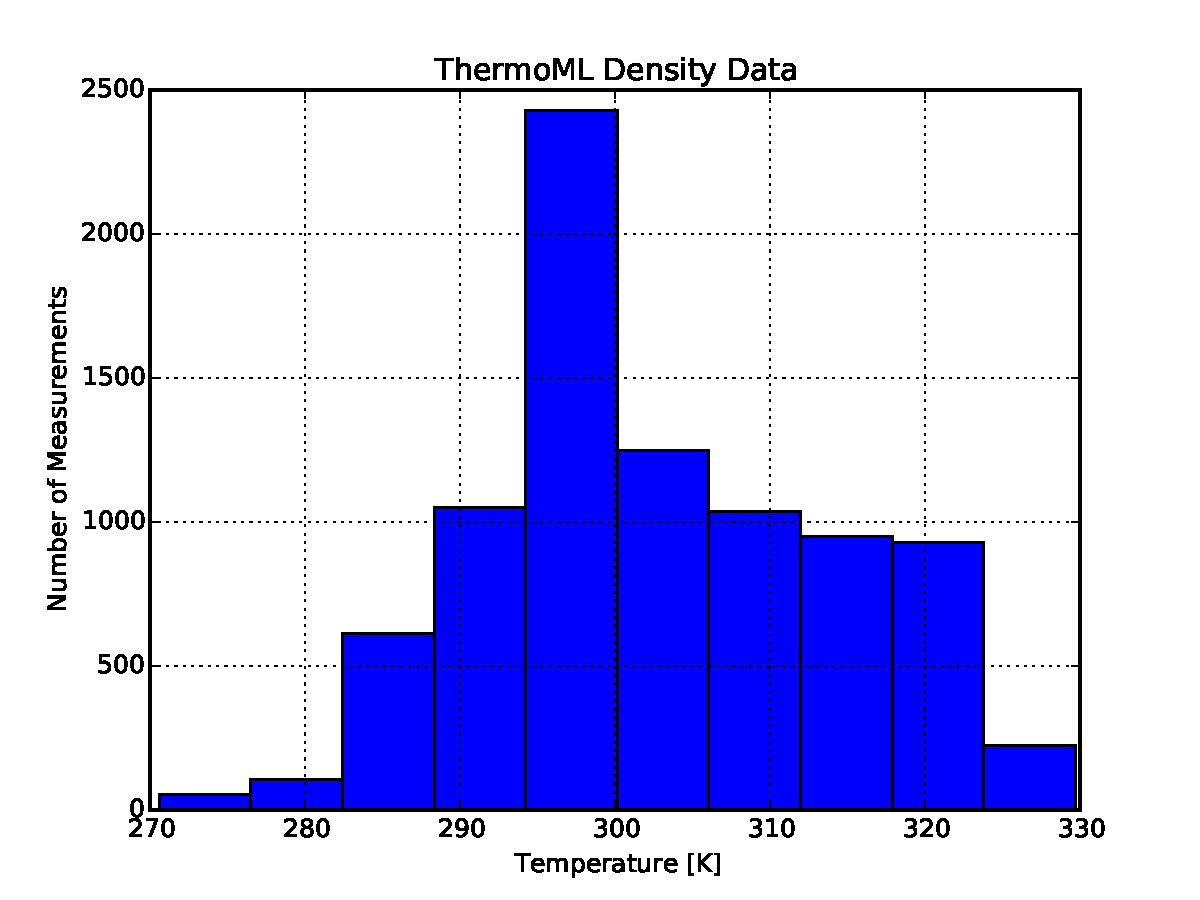
\includegraphics[width=\columnwidth]{./figures/thermoml_density_histogram.pdf}

\subsection{Benchmarking GAFF against ThermoML: Mass Density}

Mass density has been widely used as a critical ingrediant for parameterizing and testing forcefields, particularly the Lennard Jones parameters.  We therefore used the present ThermoML compilation as a benchmark of the Generalized Amber Force Field.  

\begin{figure}
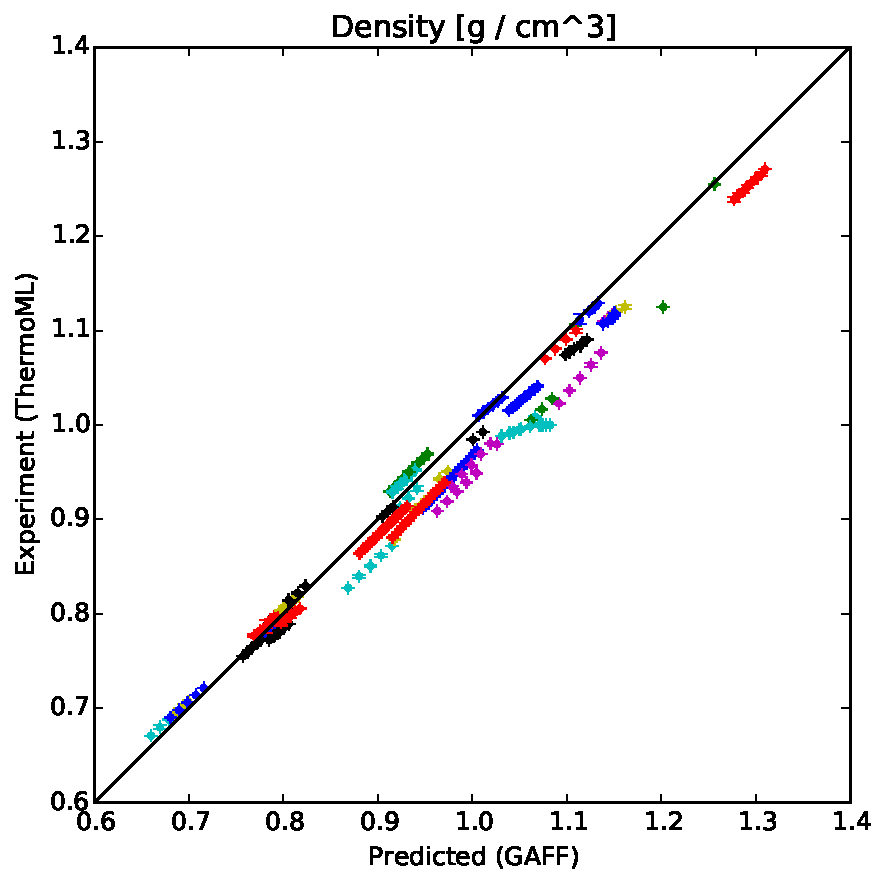
\includegraphics[width=\columnwidth]{./figures/densities_thermoml.pdf}
\caption{Density Benchmark, ThermoML+GAFF} 
\end{figure}


\subsection{Benchmarking GAFF against ThermoML: Static Dielectric}

As a measure of the electronic medium, the static dielectric constant of neat liquids provides a critical benchmark that is orthogonal to density and thermodynamic quantities.  We therefore compare our GAFF simulations against the measurements in our ThermoML compilation.  Overall, we find the dielectric constants to be qualitatively reasonable, but with clear deviations from experiment.  In particular, the nonpolar organics show a clear discrepency, with the MD predictions of 1.0 being substantially less polar than the measurements near 2.0.  Because this deviation likely stems from the lack of electronic polarization, we added a simple empirical correction for polarization \cite{bosque2002polarizabilities}, which leads to better agreement with experiment.  A similar polarization correct was used in the developemnt of the TIP4PEW water model; however, the need is much greater for the nonpolar organics, as the missing polarizability is the domimant term in the static dielectric constant.  For comparison, we also applied the same empirical correction to the VirtualChemistry dataset and saw similarly improved agreement with experiment for both the GAFF and OPLS forcefields.


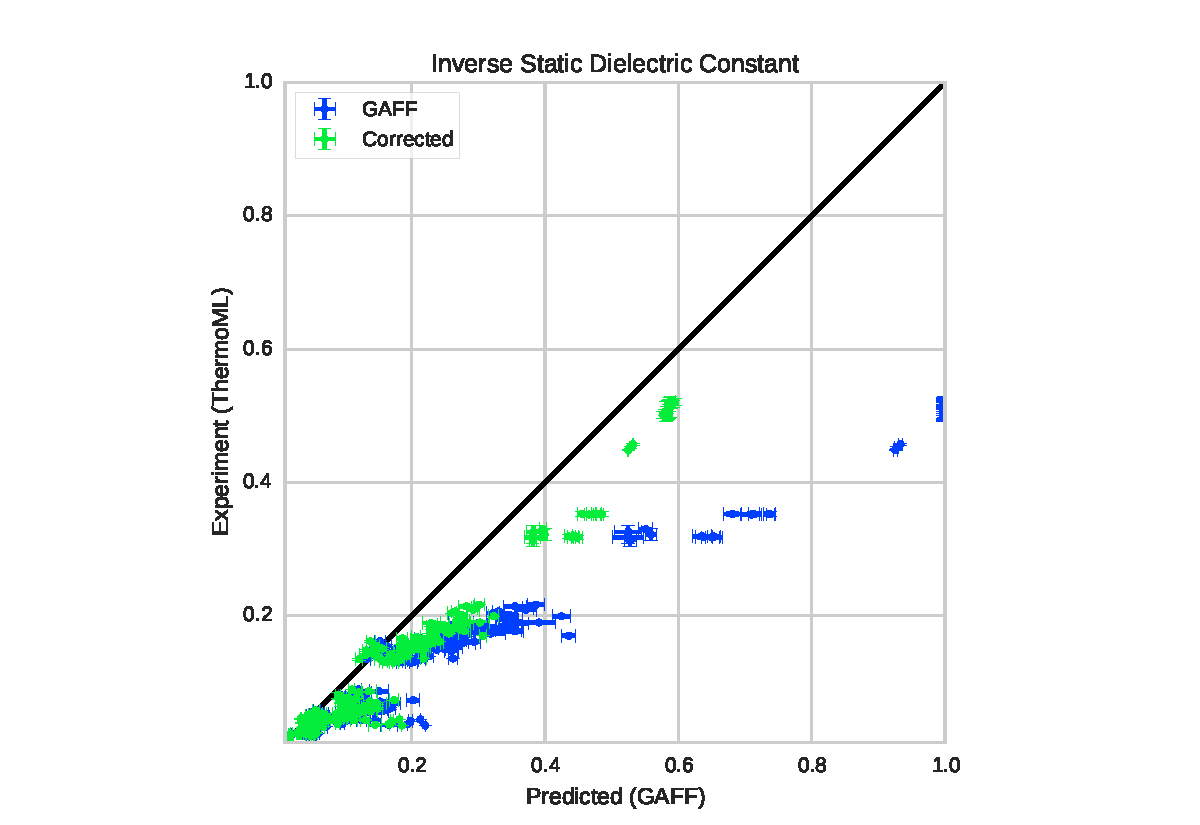
\includegraphics[width=\columnwidth]{./figures/dielectrics_thermoml.pdf}

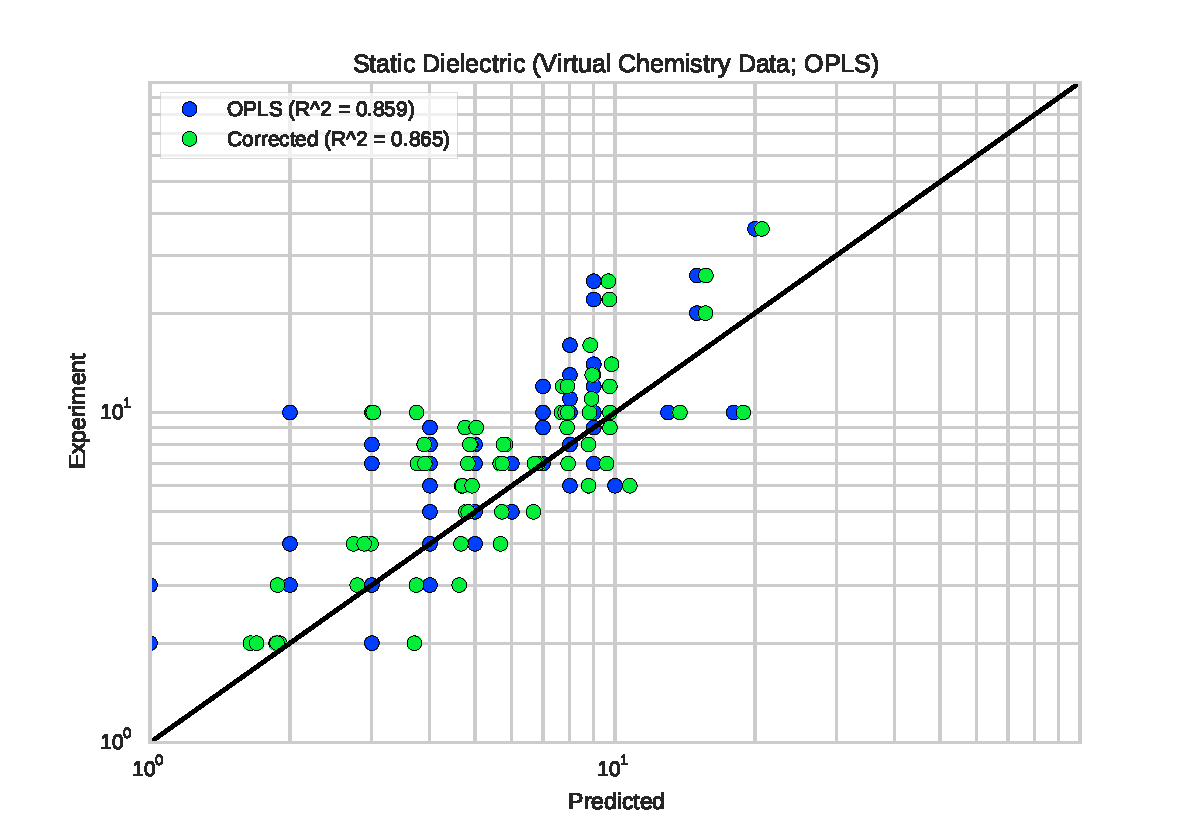
\includegraphics[width=\columnwidth]{./figures/dielectric_virtual_chemistry_opls.pdf}

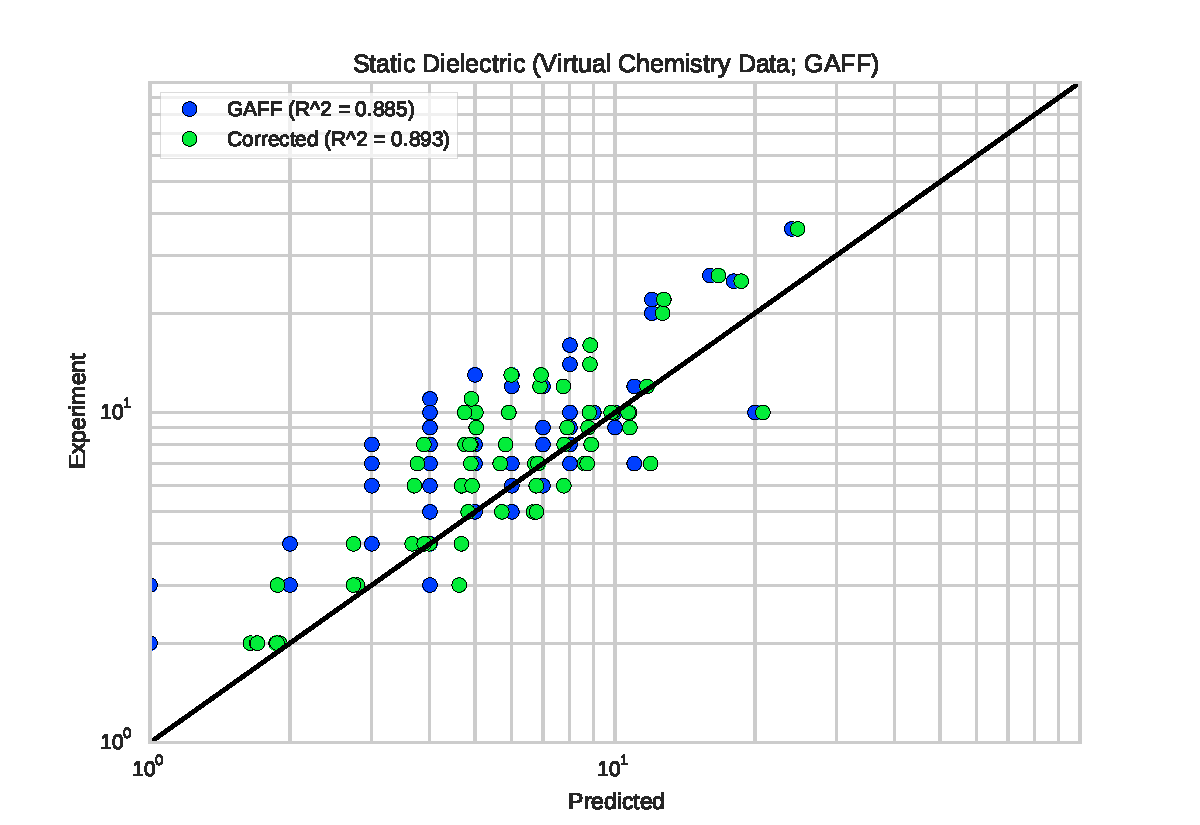
\includegraphics[width=\columnwidth]{./figures/dielectric_virtual_chemistry_gaff.pdf}

\section{Discussion}

\subsection{Forcefield Accuracy Depends on Functional Group}

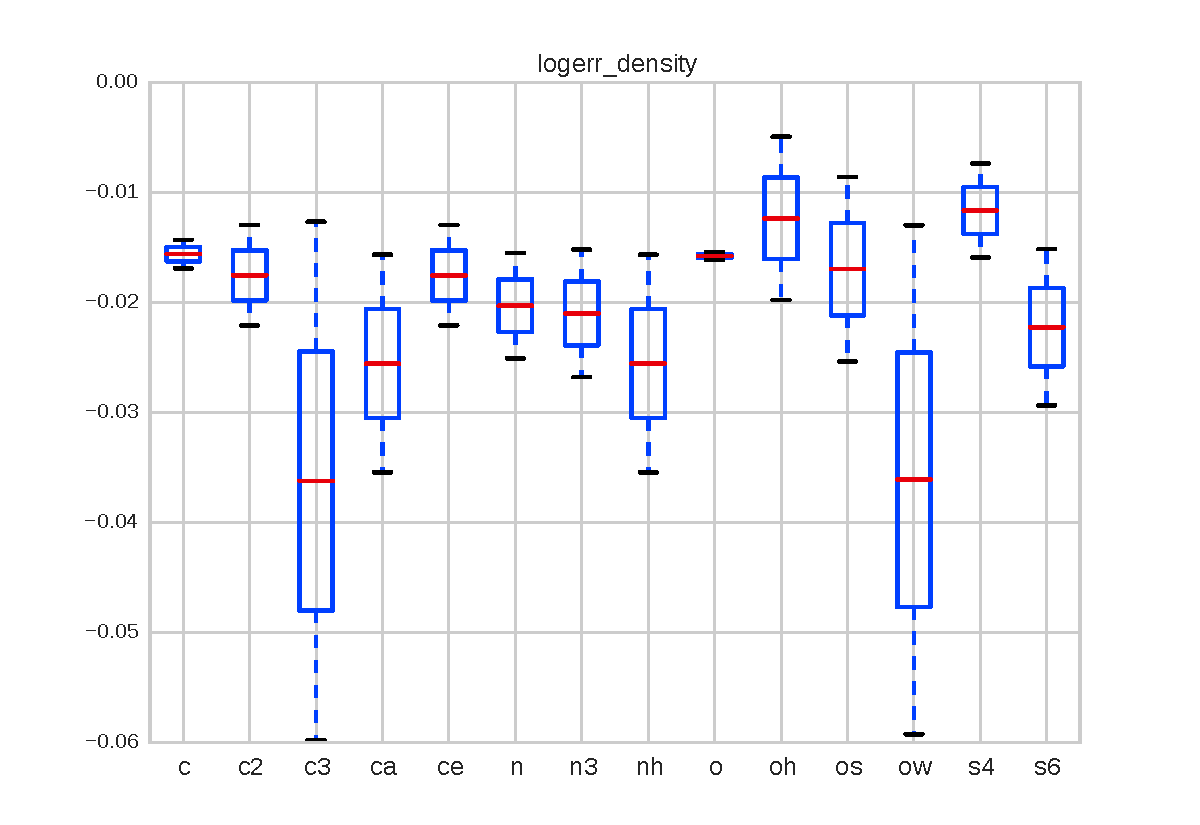
\includegraphics[width=\columnwidth]{./figures/functional_group_logerr_density.pdf}

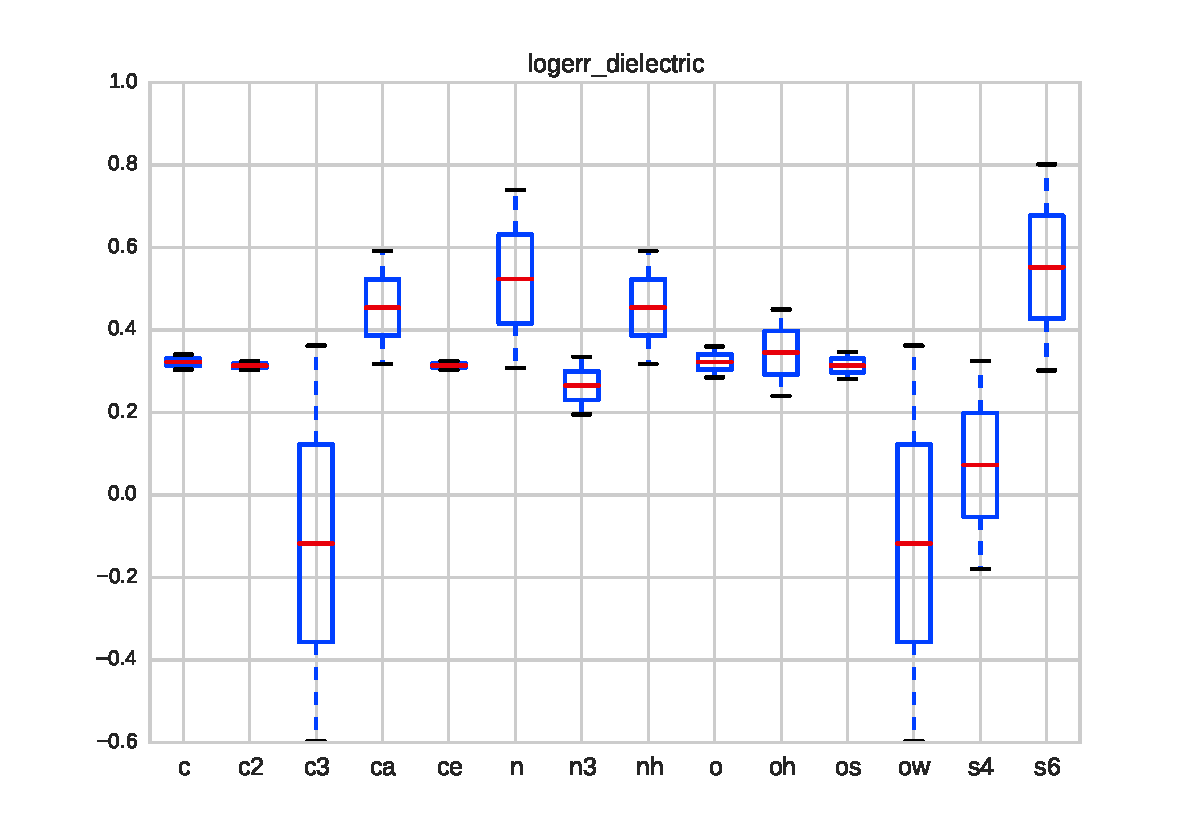
\includegraphics[width=\columnwidth]{./figures/functional_group_logerr_dielectric.pdf}

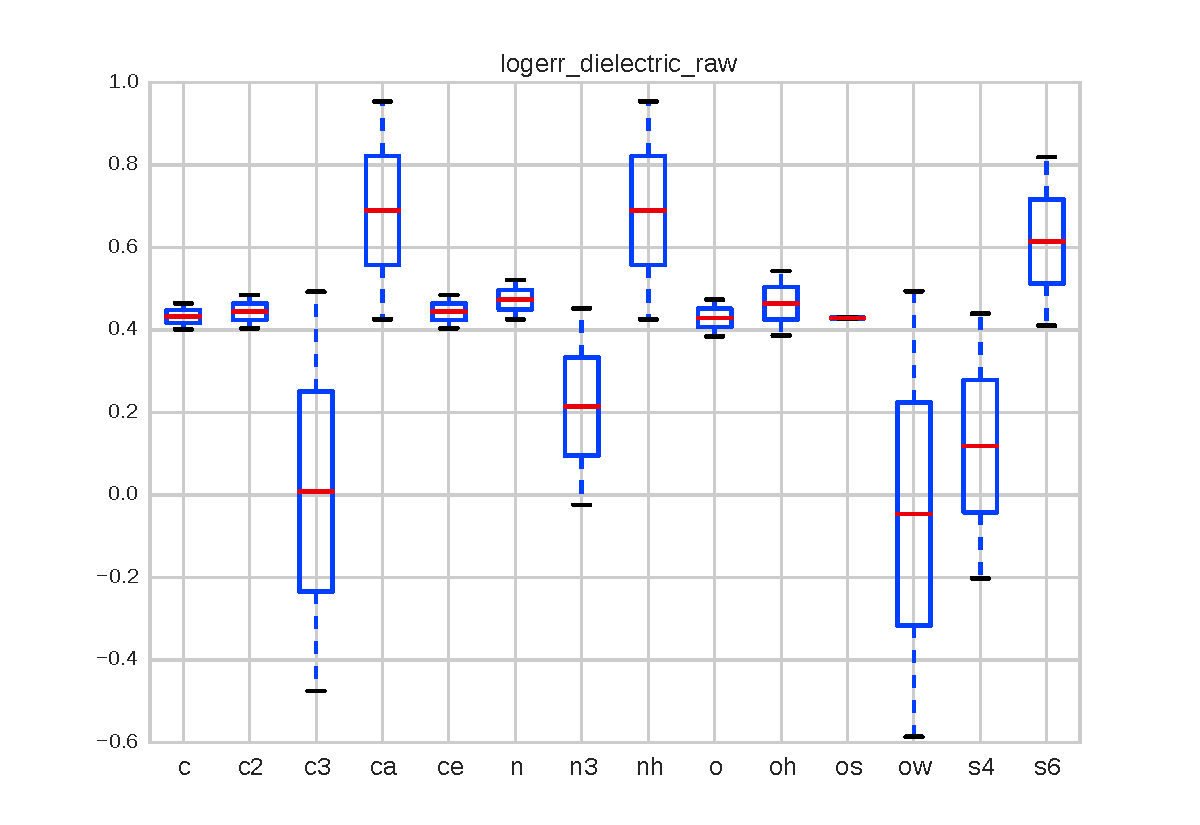
\includegraphics[width=\columnwidth]{./figures/functional_group_logerr_dielectric_raw.pdf}

\subsection{Fitting Forcefields to Dielectric Constants}

Recent forcefield development has seen a resurgence of papers fitting dielectric constants as primary data \cite{leeping, mobley}.  However, a number of authors have pointed out potential challenges in constructing self-consistent fixed-charge force fields \cite{davisguy}.  Interestingly, a recent work by Dill \cite{fennell2012simple} pointed out that, for CCL4, reasonable choices of point charges are incapable of recapitulating the observed dielectric of 2.X, instead producing dielectric constants in the range of $1.0 \le \epsilon \le 1.05$.  Suppose, for example, that one attempts to directly fit the static dielectric constants of CH4, CClH3, CCl2H2, CCl3H, CCl4.  In moving from the tetrahedrally-symmetric CCL4 to CCl3H, it suddenly becomes possible to achieve the observed dielectric constant of 2.X.  However, in the model for CCl3H, the fixed point charges are overpolarized and account for two sources of dielectric: the net dipole moment and the (electronic) polarizability.  We hypothesize that this inconsistency in parameterization may lead to strange mismatches, where symmetric molecules (e.g. benzene, CCL4) have qualitatively different properties than closely related assymetric molecules (e.g. toluene, CHCl3).  As a first-order fix, we suggest using empirical polarization corrections before directly comparing measured static dielectric constants to fixed-charge models--particularly when examining low-dielectric solvents.


\subsection{ThermoML as a Data Source}

Pro: Automated, Curated, Growing, Free, Paper trail
Cons: Requires Parsing, Data Entry Errors

\section{Methods}

\subsection{Simulation}
Boxes of 1000 molecules were constructed using PackMol \cite{}.  AM1-BCC charges were generated using the OpenEye toolkit, using the XYZ module with parameter ZYX.  The selected conformer was then processed using antechamber in AmberTools 14.  The resulting AMBER files were converted to OpenMM \cite{} XML files.  Simulation code used libraries gaff2xml (rev), trustbutverify (rev), openmm 6.2, and MDTraj \cite{} 1.2.  

Molecular dynamics simulations were performed in the NPT ensemble using a Langevin itegrator (friction 1 / picosecond?) and a Monte Carlo barostat.  Particle mesh ewald \cite{} was used with a long-range cutoff of 1.0??? nanometers.  Simulations were continued until density standard errors reached N decimals of precision, as estimated using the equilibration detection module in pymbar 2.1 \cite{}.  Trajectory analysis was performed using OpenMM \cite{} and MDTraj \cite{}.  

\section{Conclusions}

1.  ThermoML is a potentially useful resource for the forcefield community
2.  We have curated a subset of ThermoML for neat liquids with druglike atoms, with thousands of densities and hundreds of dielectrics
3.  Empirical polarization models correct a systematic bias in comparing fixed-charge forcefields to static dielectric constants


\bibliography{benchmark}

\end{document}